\chapter{Mecánica Celeste}

%%%%%%%%%%%%%%%%%%%%%%%%%%%%%%%%%%%%%%%%%%%%%%%%%%%%%%%%%%%%%%%%%%%%%%%%%%%%%%
%%%%%%%%%%%%%%%%%%%%%%%%%%%%%%%%%%%%%%%%%%%%%%%%%%%%%%%%%%%%%%%%%%%%%%%%%%%%%%
%%%%%%%%%%%%%%  PROBLEMA DE LOS DOS CUERPOS %%%%%%%%%%%%%%%%%%%%%%%%%%%%%%%%%%
%%%%%%%%%%%%%%%%%%%%%%%%%%%%%%%%%%%%%%%%%%%%%%%%%%%%%%%%%%%%%%%%%%%%%%%%%%%%%%
%%%%%%%%%%%%%%%%%%%%%%%%%%%%%%%%%%%%%%%%%%%%%%%%%%%%%%%%%%%%%%%%%%%%%%%%%%%%%%

\section{Problema de los dos cuerpos}


\subsection{Leyes de Kepler}

Podríamos decir que el problema de los dos cuerpos comienza con la formulación de las tres leyes para el movimiento planetario por parte de Kepler. Estas tres leyes trataban de dar cuenta sobre como se movían los astros alrededor del Sol, y entonces los primeros pasos para la descripción de los cuerpos celestes:

\begin{itemize}
	\item \textbf{Ley de las órbitas}: los planetas se mueven en órbitas elípticas, con el Sol en uno de los focos de la elipse.
	\item \textbf{Ley de las áreas}: la línea que conecta un planeta y el Sol barre áreas iguales en tiempos iguales.
	\item \textbf{Ley de períodos}: el cuadrado del período orbital de un planeta ($T$) es proporcional al cubo del a distancia media del planeta al Sol:
	      \begin{equation}
		      T^2 = \frac{4\pi^2}{\mu}a^3
	      \end{equation}
	      donde $a$ es el semi-eje mayor de la elipse, que es igual al promedio entre las distancias en perihelio $r_p$ y afelio $r_a$\footnote{Más tarde definiremos mejor que es un afelio y perihelio, pero dicho rápidamente, el afelio es el punto de la órbita del planeta más alejado del Sol, y el perhelio el punto más cercano.}
\end{itemize}

\subsection{Ecuaciones diferenciales fundamentales}

El \textit{problema de los dos cuerpos} o \textit{problema de Kepler} es el nombre que se le da al problema de la dinámica de dos cuerpos celestes (suponiendo que estos están completamente aislados). Este problema hoy en día esta asociado a 6 ecuaciones diferenciales no linales, autónomas\footnote{Que una ecuación diferencial sea autónoma significa que no depende explícitamente de la coordenada diferencial, en nuestro caso, el tiempo.} de segundo orden, las cuales vienen dadas en última instancia por la \textit{ley de gravitación universal de Newton}. Estas ecuaciones diferenciales son:

\begin{equation}
	\left\lbrace
	\begin{split}
		m_1 \ddot{\rn}_1 \ = \  & \frac{Gm_1m_2}{r^2} \frac{\rn_2-\rn_1}{r} \\
		m_2 \ddot{\rn}_2 \ = \  & \frac{Gm_1m_2}{r^2} \frac{\rn_1-\rn_2}{r}
	\end{split} \right.
\end{equation}
donde $\rn_1$ es la posición del cuerpo de masa $m_1$, $\rn_2$ la posición del cuerpo de masa $m_2$ y $r=|\rn|=|\rn_1-\rn_2|$ la distancia entre los dos cuerpos. Para resolver este problema de manera analítica se suele usar un cambio de variables muy sencillo:

\begin{equation}
	\rn_c = \frac{m_1\rn_1+m_2\rn_2}{m_1+m_2} \tquad \rn=\rn_1-\rn_2
\end{equation}
tal que $\rn_c$ es la \textit{posición del centro de masas} y $\rn$ es la \textit{posición reducida}. Veamos que este cambio de coordenadas es invertidble:

\begin{equation}
	\rn_1 = \rn_c + \frac{m_2}{m_2+m_1} \rn  \tquad \rn_2 = \rn_c - \frac{m_1}{m_2+m_1} \rn
\end{equation}
Una vez fijamos el nuevo sistema llamado \textbf{sistema reducido}, tenemos que las ecuaciones diferenciales pasan a ser mucho más sencilas:

\begin{equation}
	\ddot{\rn}_c  =  \quad 0 \tquad
	\ddot{\rn}  = - \frac{\mu}{r^3} \rn
\end{equation}
donde $\mu$ es la llamada \textit{masa reducida} y se define como $\mu = G (m_1+m_2)$. a primera ecuación tiene una solución extremadamente sencilla $\rn_c(t)=a+bt$, y esta nos lleva a la conservación de las cantidades \textit{momento total} $\Pn$ y \textit{momento angular total} $\Ln$, definidos como
\begin{equation}
	\Pn = \pn_1 + \pn_2 \tquad \Ln = \rn_1 \wedge \pn_1 + \rn_2 \wedge \pn_2
\end{equation}
donde $\pn=m\vn=m\dot{\rn}$. Siempre podemos encontrar un sistema de referencia donde el centro de masas está quieto, tal que $\Pn=0$. A este sistema de referencia lo llamamos \textit{sistema de referencia del centro de masas}, y lo que nos dice es que $\rn_c(t)=0$, y por tanto que el movimiento de $\rn_1$ y $\rn_2$ está determinado únicamente por su movimiento relativo $\rn$. A la hora de describir la órbita de dos cuerpos este es el sistema de referencia mas usado, por ser el más sencillo.

\subsection{Solución de la ecuación reducida}

El problema de los dos cuerpos se reduce ahora a obtener la solución de la ecuación reducida

\begin{equation*}
	\ddot{\rn} = - \frac{\mu}{r^3} \rn \qquad \rn=\rn_1-\rn_2 \qquad \mu=G(m_1+m_2)
\end{equation*}
Estas 3 ecuaciones diferenciales de grado 2 se pueden expresar como 6 ecuaciones diferenciales de grado 1, tales que

\begin{equation}
	\left\lbrace \
	\begin{split}
		\dot{\rn} \ = \  & \vn                   \\
		\dot{\vn} \ = \  & - \mu \frac{\rn}{r^3}
	\end{split}
	\right.
\end{equation}
Para solucionar estas ecuaciones diferenciales lo que haremos es suponer que existen varias cantidades conservadas (las cuales efectivamente se cosnervarán). Estas cantidades conservadas son:

\begin{itemize}
	\item \textbf{Momento angular}: $\cn=\rn\wedge\vn$.
	\item \textbf{Energía}: $h=\frac{v^2}{2}-\frac{\mu}{r}$.
	\item \textbf{Vector excéntrico}: $\en=\frac{1}{\mu} \vn \wedge \cn - \frac{\rn}{r}$.
\end{itemize}
Estas cantidades representan un total de siete constantes del movimiento. Sin embargo, no son completamente independientes, ya que están ligadas por al menos dos relaciones fundamentales:

\begin{itemize}
	\item Ortogonalidad entre el momento angular y el vector excétrico
	      \begin{equation}
		      \mathbf{c} \cdot \mathbf{e} = 0.
	      \end{equation}

	\item Relación entre la excentricidad, energía y momento angular.
	      \begin{equation}
		      e^2 = \frac{2hc^2}{\mu^2} + 1
	      \end{equation}
	      siendo $c$ el módulo de $\cn$ y $e$ el módulo de $\en$, al que se le llama \textbf{excentricidad}.
\end{itemize}
Debido a estas restricciones, el número de grados de libertad efectivos en el problema de la masa reducida se reduce a cinco, con un parámetro libre que definirá nuestra órbita, a saber, un ángulo. Antes de hablar del ángulo debemos definir el plano en el que dicho ángulo es un ángulo polar, el cual será evidente: si $\cn$ se conserva, la posición $\rn$ y velocidad $\vn$ de neustra partícula virtual forman un plano en el que el movimiento de la masa reducida está restringida. Este plano se llama \textit{plano orbital}, y el movimiento de las partículas 1 y 2 están restrigidas a este plano, y por tanto el movimiento reducido depende de dos coordenadas, de la distancia al punto cero del sistema de referencia (que en general será $\rn_c=0$) y el ángulo con un eje de dicho plano (un eje arbitrariamente elegido). Dado que $\cn \times \en = 0$, podemos afirmar que el vector excéntrico $\en$ vive en el plano orbital, y como no varía con el tiempo, es un buen eje para tomarlo como eje de referencia. En general este vector se suele elegir como el ángulo el conformado por $\rn$ y $\en$, que llaremos \textbf{anomalía verdadera}.

\begin{equation}
	\cos (f) = \frac{\rn \cdot \en}{|\rn||\en|}
\end{equation}
Una vez tenemos todo esto la ecuación diferencial del vector posición reducido tiene la siguiente solución

\begin{equation}
	\rn(f) = \frac{c^2/\mu}{1+e\cos(f)}
\end{equation}
\hspace{-0.0mm} \vspace{1.0mm} \begin{minipage}{0.55\textwidth}
	A  la cantidad $l=c^2/\mu$ la llamamos \textit{semilatus rectum} se define como la distancia para la cual $f=\pi/2$. En el caso de una elipse, esta distancia se puede entender como la distancia que hay entre uno de los focos de la elipse y la elipse en una línea perpendicular al semieje mayor. Esta definición es un poco liosa, por eso recomendamos ver el dibujo. La distancia entre el centro y la masa reducida también depende de la anomalía verdadera, y la excentricidadde, que define el tipo de órbita que seguirá nuestra partícula. Las trayectorias son cónicas, tales que:
\end{minipage}	\hfill
\begin{minipage}{0.47\textwidth}
	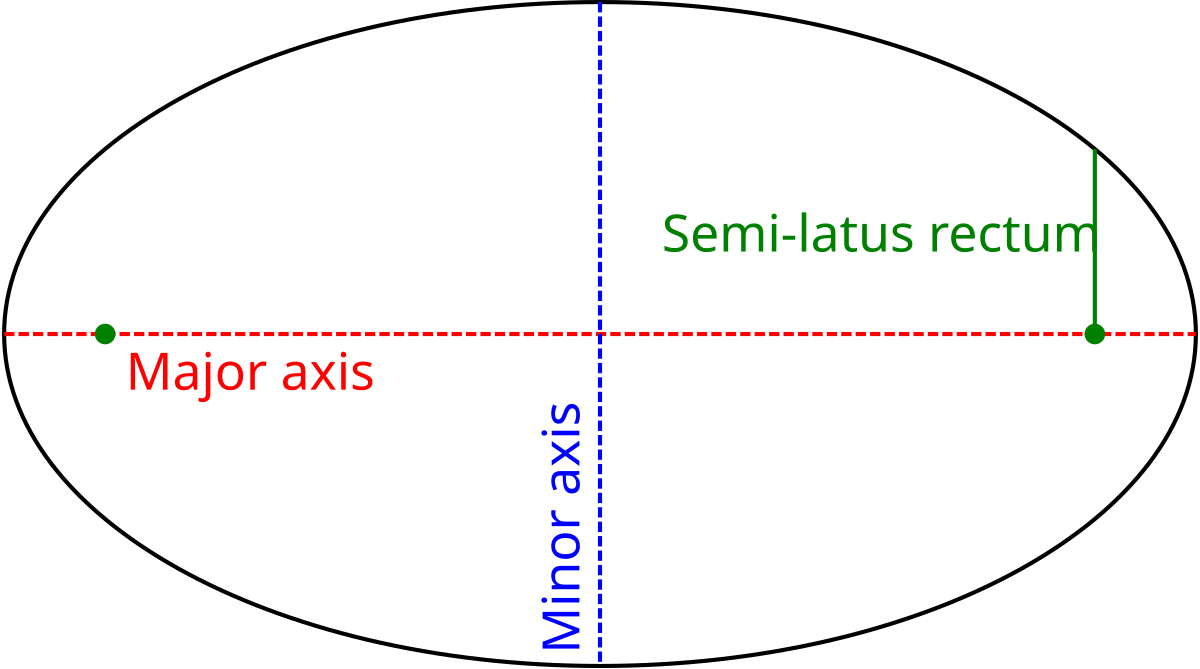
\includegraphics[width=0.9\textwidth]{Cuerpo/Ch_02/02_Semilatus_rectum.png}
\end{minipage}


\begin{itemize}
	\item \textbf{Trayectoria circular}: ocurre cuando $e=0$, tal que $r=l$.
	\item \textbf{Trayectoria elíptica}: ocurre cuando $e=0$. En este caso aparecen lo que llamamos la \textit{periapsis}, que es la distancia más pequeña a la que se puede encontrar nuestra partícula reducida del centro del SR, tal que $r_{per}=l/(1+e)$; y la \textit{apoapsis} que es la distancia más grande a la que se puede encontrar nuestra partícula del centro del, tal que $r_{ap}=l/(1-e)$. Cuando estos términos se refieren a la trayecotia de la tierra sobre el sol las llamamos perigeo y apogeo, y cuando es de un planeta cualquiera respecto al sol decimos perihelio y apohelio.
	\item \textbf{Trayecotria hiperbólica}: ocurre cuando $e=1$.
	\item \textbf{Trayecotia parabólica}: ocurre cuando $e>1$.
\end{itemize}
-
\begin{figure}[h!] \centering
	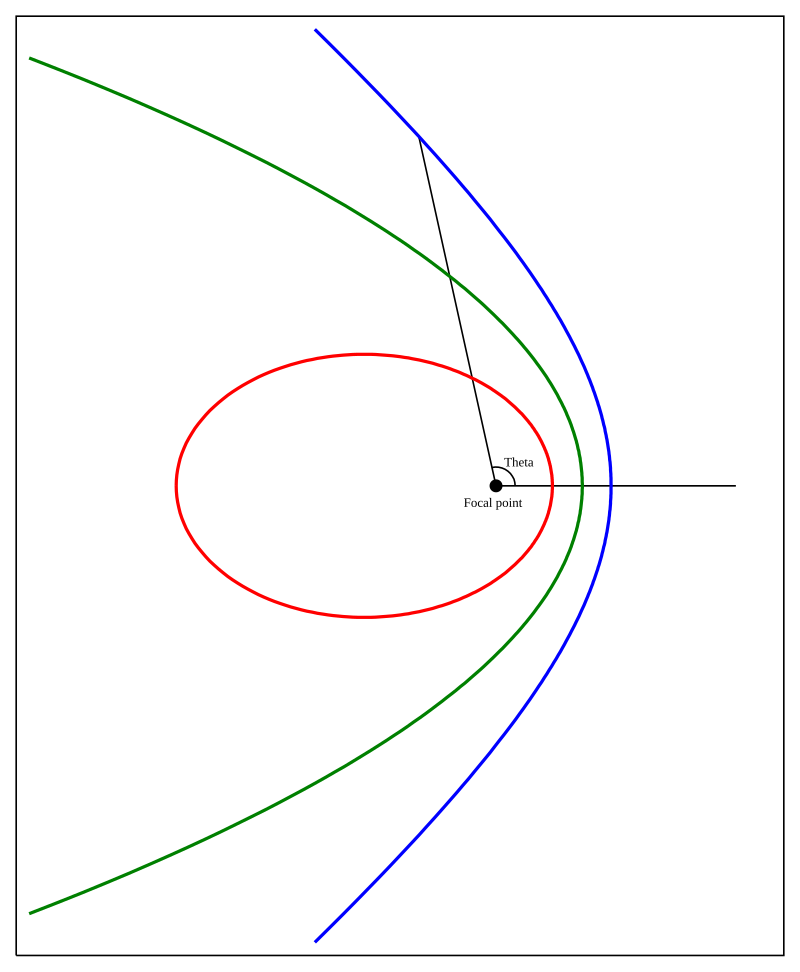
\includegraphics[width=0.5\linewidth]{Cuerpo/Ch_02/02_Kepler_Orbits.png}
	\caption{Órbitas de Kepler en función de la excentricidad. En color \textcolor{red}{rojo} $e=0.7$, en color \textcolor{green}{verde} $e=1$ y en color \textcolor{blue}{azul} $e=1.3$. Imagen de la \href{https://es.wikipedia.org/wiki/Excentricidad_orbital}{Wikipedia}.}
\end{figure}

\subsection{Plano orbital en función de otro plano de referencia}

Como hemos visto, los cuerpos se mueven en el llamado plano orbital. Su movimiento, en este plano, depende de 3 parámetros: el momento angular $\cn$ (el cual define la dirección del plano y el \textit{semilatus rectum}), la anomalía verdadera $f$\footnote{Se emplea el tiempo de paso por el periastro $\tau$, la anomalía media $M$ y la longtidu media $L$.} y el valor de la excentricidad $e$.  Sin embargo nosotros no usaremos como referencia el plano orbital, sino otro. Para definir el plano orbital respecto al \textit{plano de referencia} (esto es, el eje de coordenadas), usamos 3 coordenadas, para las cuales es importante definir el \textit{vector nodo ascendente} $\Nn=\hnz\wedge\cn$. Este vector define lo que llamamos el punto nodo ascendente, y está contenido tanto en el plano orbital como en el plano de referencia. Las 3 coordenadas:
\begin{itemize}
	\item \textbf{Inclinación} ($i$): ángulo entre el plano de la órbita y el plano referencia.
	      \begin{equation}
		      \cos (i) = \frac{\cn \cdot \hnz}{|\cn||\hnz|}
	      \end{equation}
	\item \textbf{Longitud del nodo ascendente} ($\Omega$). Ángulo medido en plano de referencia desde la dirección de referencia hasta la dirección del nodo ascendente:
	      \begin{equation}
		      \cos (\Omega) = \frac{\Nn \cdot \hnx}{|\Nn||\hnx|}
	      \end{equation}
	\item \textbf{Argumento del periastro} ($\omega$). Ángulo medido en el plano de la órbita desde la dirección del nodo ascendente hasta el periastro.
	      \begin{equation}
		      \cos (\omega) = \frac{\Nn \cdot \en}{|\Nn||\en|}
	      \end{equation}
\end{itemize}
\begin{figure}[h!] \centering
	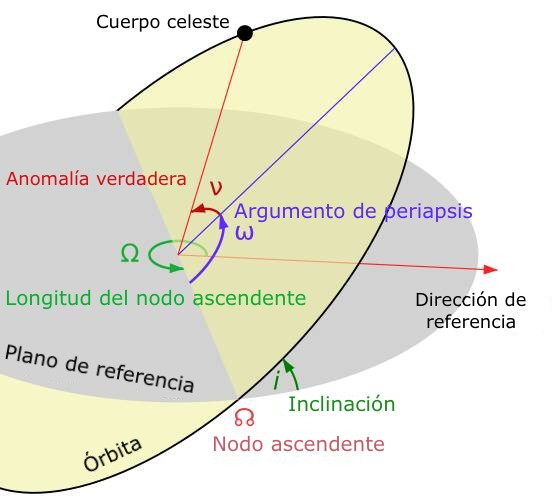
\includegraphics[width=0.6\linewidth]{Cuerpo/Ch_02/02_Elementos_orbitales.jpg}
	\caption{Definición de los 3 parámetros necesarios para describir un plano orbital en el de referencia.}
\end{figure}
\subsection{Relaci\'on entre las anomal\'ias orbitales}

En mec\'anica celeste, es fundamental entender distintos \'angulos que describen la posici\'on de un cuerpo en su \'orbita alrededor de un foco. Cada uno de estos \'angulos tiene un significado f\'isico particular y es \'util en distintos contextos del estudio de las \'orbitas. 

\subsubsection{Anomal\'ia exc\'entrica ($E$)}
La anomal\'ia exc\'entrica $E$ es un \'angulo auxiliar que permite traducir la posici\'on de un cuerpo en una \'orbita el\'iptica a una posici\'on equivalente en un c\'irculo auxiliar. Se usa para facilitar los c\'alculos matem\'aticos en las ecuaciones de Kepler, ya que describe el movimiento de un punto ficticio que se mueve con velocidad angular uniforme.

\subsubsection{Anomal\'ia media ($M$)}
La anomal\'ia media $M$ representa un \'angulo ficticio que describe el avance de un cuerpo en su \'orbita suponiendo que se mueve a velocidad angular constante. Es decir, no refleja directamente la posici\'on real del cuerpo, sino una versi\'on simplificada que facilita los c\'alculos de tiempo y evoluci\'on orbital. Se mide a partir del periastro $\tau$ y se usa en la ecuaci\'on de Kepler para determinar la posici\'on real del cuerpo en cada instante de tiempo.

\subsubsection{Longitud media ($L$)}
La longitud media $L$ es la suma de la anomal\'ia media $M$ y la longitud del periastro, es decir:

\begin{equation}
    L = M + \varpi.
\end{equation}

F\'isicamente, la longitud media proporciona una forma conveniente de expresar la posici\'on promedio del cuerpo en la \'orbita sin depender de la excentricidad de esta. Se usa en c\'alculos de efem\'erides y en la predicci\'on de posiciones orbitales a largo plazo.

\subsubsection{Significado f\'isico y aplicaci\'on}
Cada una de estas anomal\'ias es clave para la descripci\'on y predicci\'on del movimiento orbital. Mientras que la anomal\'ia verdadera da la posici\'on real del cuerpo en su \'orbita, la anomal\'ia media y la longitud media permiten reformular el problema en t\'erminos matem\'aticos m\'as simples, facilitando as\'i el c\'alculo de trayectorias y tiempos de paso por ciertos puntos de la órbita. Esto es fundamental en la astrodin\'amica para la navegaci\'on espacial y la predicci\'on de efem\'erides de cuerpos celestes.



\begin{Anotacion}
	\textcolor{red}{Hizo todo el cálculo sobre como obtener $\en$ (demostración de que se conserva), como obtener $e$ y su relación con la energía (fácil, pero zzz).}
\end{Anotacion}
\begin{Anotacion}
	\textcolor{red}{Tambíen hizo un dibujo, donde el eje x es la energía, el eje y el momento angular, y reprsento cual es el tipo de órbita en función de la región de dicho espacio de fases (elíptico, hiperbólico, parabólico, colisión...)}
\end{Anotacion}
\begin{Anotacion}
	\textcolor{red}{ Se está centrnado bastante en las características de la anomalía media (dice que varía a velocidad constante). Hablar de las demas cosas, significado, uso, razón. (Video de true anomaly vs mean anomaly), así vemos la relación entre ellas. }
\end{Anotacion}

%%%%%%%%%%%%%%%%%%%%%%%%%%%%%%%%%%%%%%%%%%%%%%%%%%%%%%%%%%%%%%%%%%%%%%%%%%%%%%%
%%%%%%%%%%%%%%%%%%%%%%%%%%%%%%%%%%%%%%%%%%%%%%%%%%%%%%%%%%%%%%%%%%%%%%%%%%%%%%%
%%%%%%%%%%%%%%  PROBLEMA DE LOS TRES CUERPOS  %%%%%%%%%%%%%%%%%%%%%%%%%%%%%%%%%
%%%%%%%%%%%%%%%%%%%%%%%%%%%%%%%%%%%%%%%%%%%%%%%%%%%%%%%%%%%%%%%%%%%%%%%%%%%%%%%
%%%%%%%%%%%%%%%%%%%%%%%%%%%%%%%%%%%%%%%%%%%%%%%%%%%%%%%%%%%%%%%%%%%%%%%%%%%%%%%

\section{Problema de los tres cuerpos}

\subsection{Introducción}

Se le llama al problema de los tres cuerpos al problema de la dinámica de tres masas $m_1,m_2$ y $m_3$ que se mueven por la acción gravitacional mutua entre ellos. En general este probema no tiene solución analítica, dado que el número de incógnitas es mayor que el número de ecuaciones que podemos emplear.

\subsection{Problema de los tres cuerpos restringido y puntos de Lagrange}

El problema restringido o problema de euler al problema de la dinámica de 3 cuerpos en el que despreciamos el efecto gravitacional sobre los otros dos, que orbitan entre sí. Esto se puede hacer cuando una de las masas es mucho menor que las otras dos (los llamados \textit{cuerpos primarios}) $m_1,m_2\gg m_3$. Un ejemplo de un cuerpo al que se le podría aplicar este tipo de dinámica es a un asteroide en el sistema solar donde $m_1$ y $m_2$ son el Sol y Júpiter. Este problema sí que es intregable, y se obtiene a partir de los siguientes pasos:

\begin{itemize}
	\item Se considera que los cuerpos masivos $m_1$ y $m_2$ se mueven en órbtia circular alrededor de su centro de masas $(O)$ y en el mismo plano de movimiento. Obtenemos la dinámica de ambos cuerpos.
	\item Luego obtenemos la posición y velocidad de $m_3$ a partir de las posiciones y velocidades de $m_1$ y $m_2$ en cada momento.
\end{itemize}
En el el problema de los tres cuerpos restringido aparecen 5 puntos de equilibrio (en un instante dado). A estos puntos se le llaman \textit{puntos de Lagrange}, y los dividimos en 2 tipos:

\begin{itemize}
	\item \textit{Colineales}: $L_1,L_2$ y $L_3$. Son inestables tipo \textit{silla}, también poseen una parte tipo \textit{centro}, que se emplea para situar satélites. En el caso Sol-Tierra econtramos por ejemplo el telescopio James Webb en $L_2$ o la sonda SOHO en $L_1$.
	\item \textit{Triangulares}: $L_4$ y $L_5$. Son estables siempre que se verifique $\mu=m_2/(m_1+m_2)<0.0385$ (cuando $m_1>m_2$) son linealmente estables, en caso contrario, son inestables. Cuando son estables (por ejemplo, Sol-Júpiter) encontramos asteroides confinados en estos puntos. También podemos encontrar algunos asteroides en los sistemas Sol-Tierra o Sol-Marte.
\end{itemize}





%%%%%%%%%%%%%%%%%%%%%%%%%%%%%%%%%%%%%%%%%%%%%%%%%%%%%%%%%%%%%%%%%%%%%%%%%%%%%%%%
%%%%%%%%%%%%%%%%%%%%%%%%%%%%%%%%%%%%%%%%%%%%%%%%%%%%%%%%%%%%%%%%%%%%%%%%%%%%%%%%
%%%%%%%%%%%%%%  EJERCICIOS %%%%%%%%%%%%%%%%%%%%%%%%%%%%%%%%%%%%%%%%%%%%%%%%%%%%
%%%%%%%%%%%%%%%%%%%%%%%%%%%%%%%%%%%%%%%%%%%%%%%%%%%%%%%%%%%%%%%%%%%%%%%%%%%%%%%
%%%%%%%%%%%%%%%%%%%%%%%%%%%%%%%%%%%%%%%%%%%%%%%%%%%%%%%%%%%%%%%%%%%%%%%%%%%%%%%

\section{Ejercicios}

\tcbstartrecording
\begin{texercise}

	Prueba que el vector excentricidad, o eje excéntrico, $\vec{e} = \frac{1}{\mu} (\vec{v} \wedge \vec{c}) - \frac{\vec{r}}{r}$, lleva sentido hacia la periapsis.
	\tcblower
	Tenemos que demostrar que el vector excentricidad lleva el sentido hacia la periapsis.


	\begin{minipage}{.45\textwidth}
		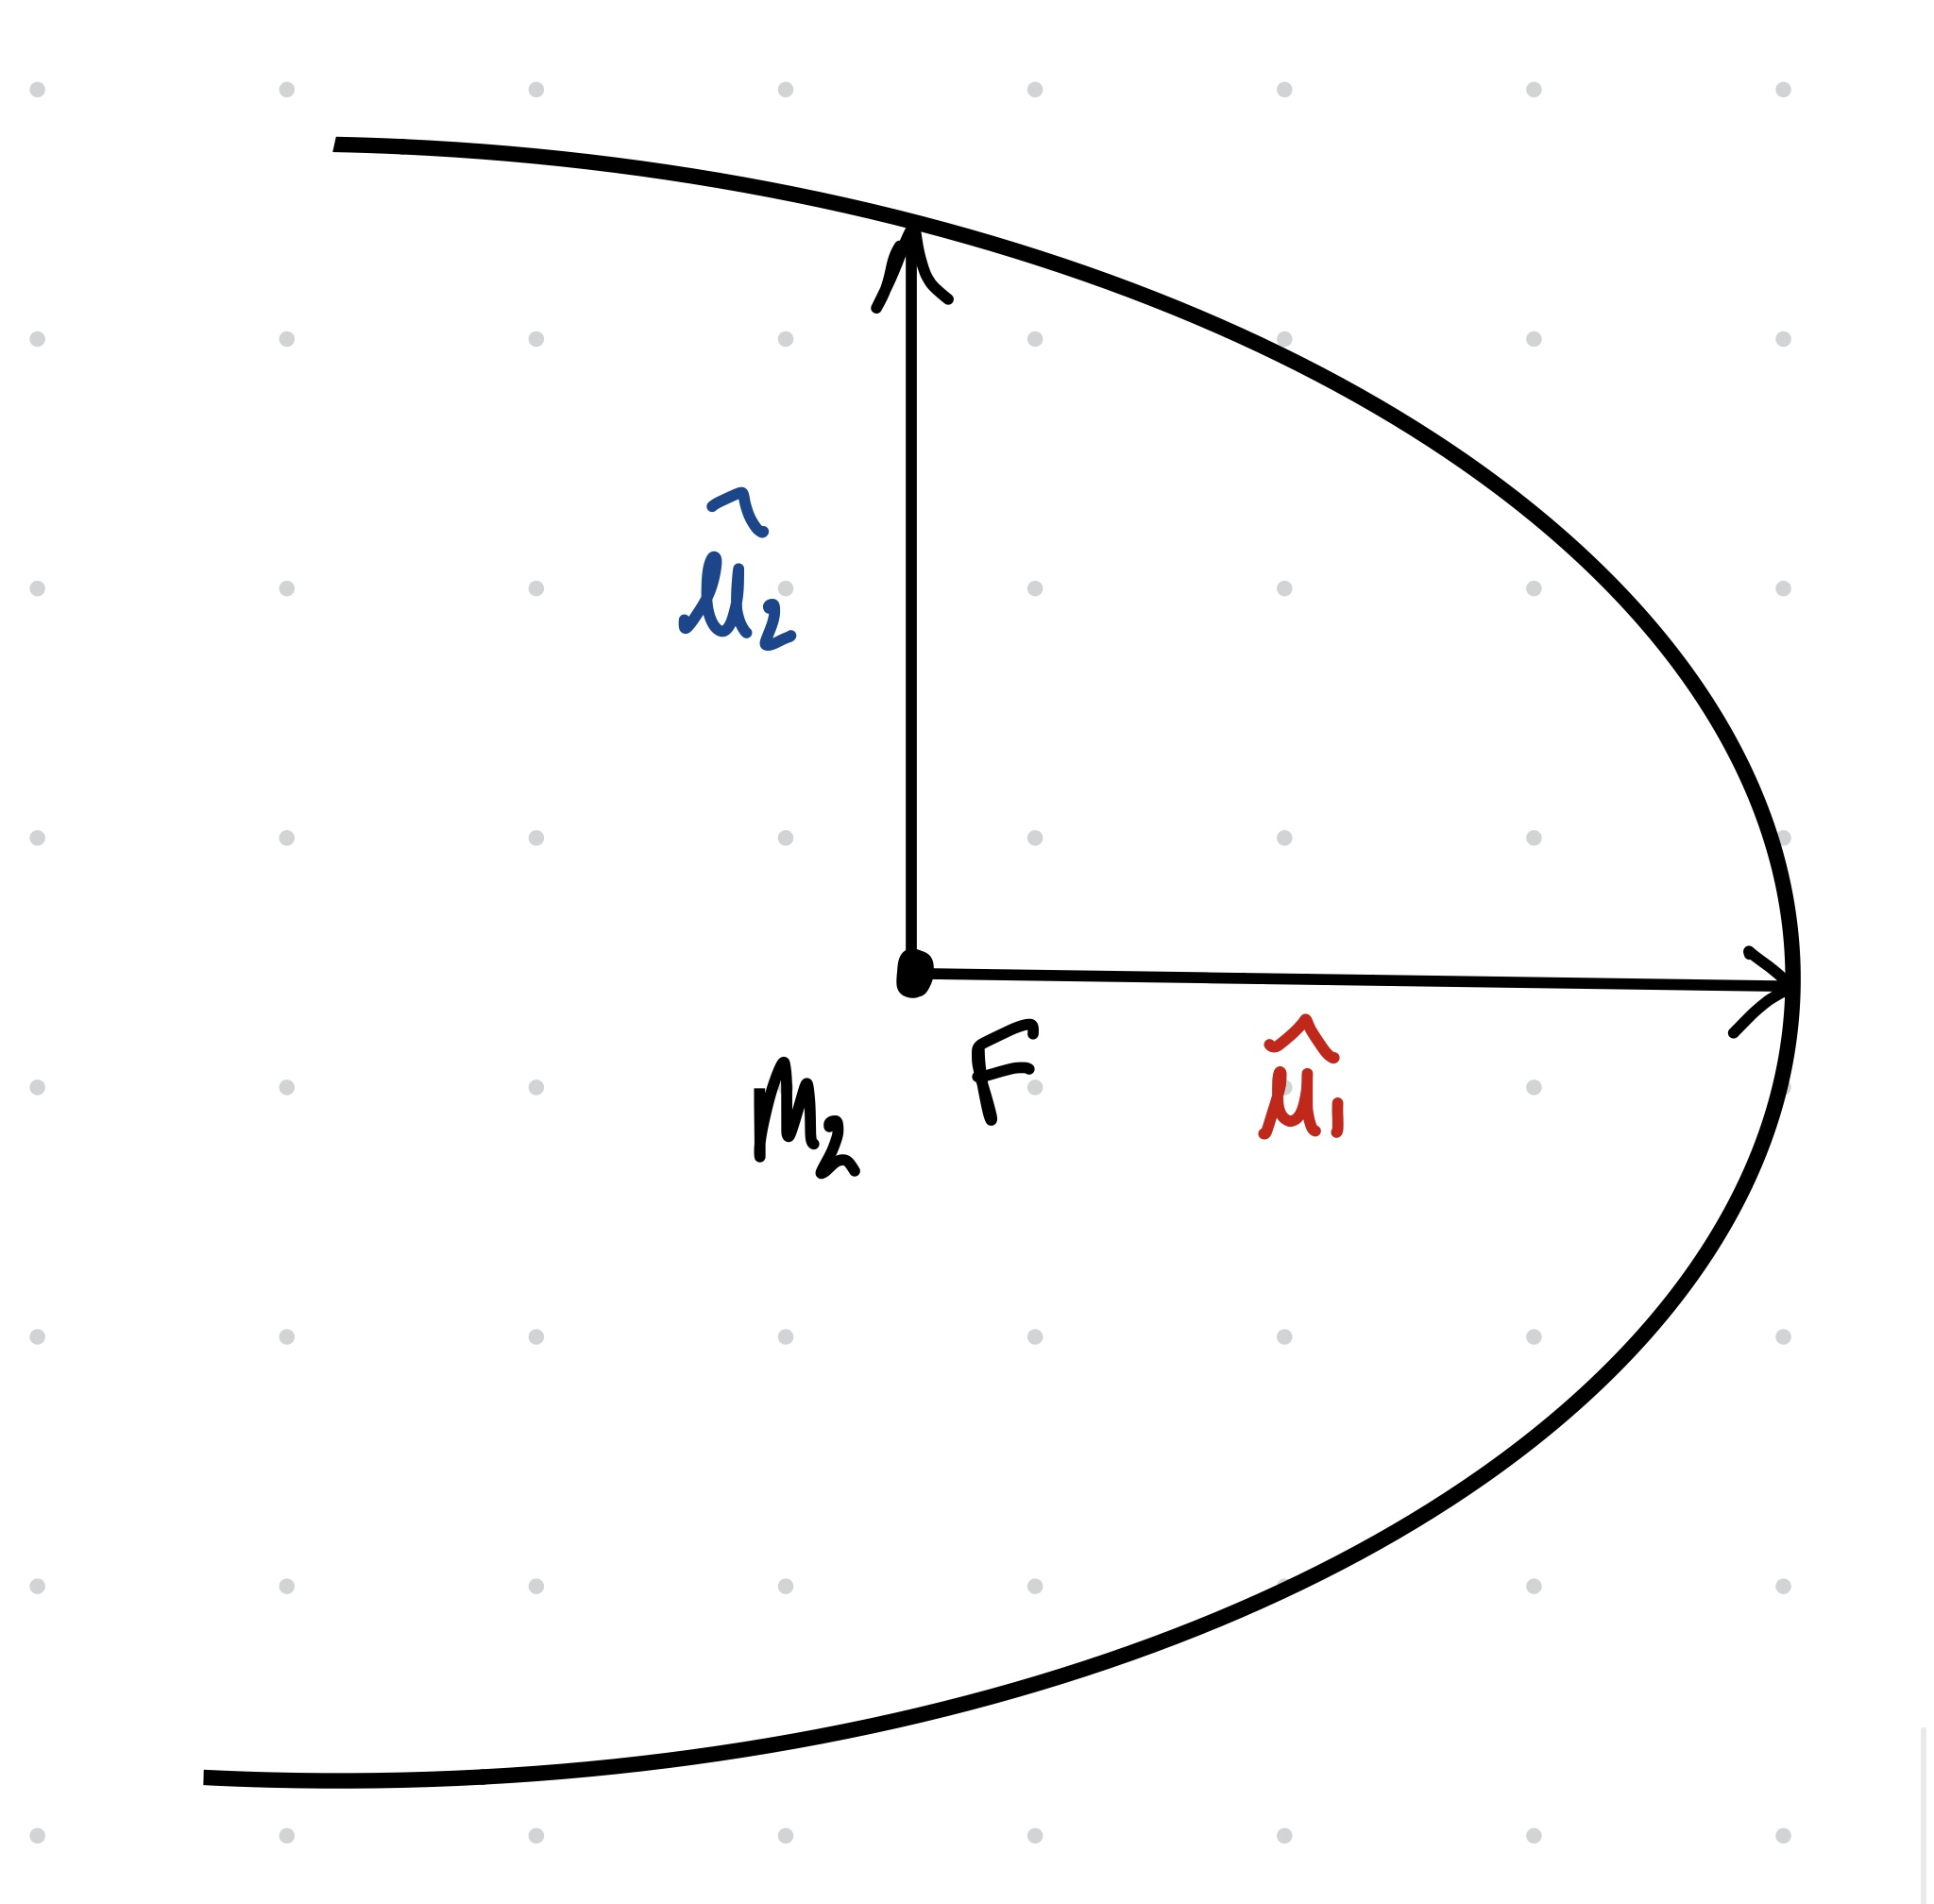
\includegraphics[width=0.8\textwidth]{Cuerpo/Imagenes/02_Ejercicio_1_1.jpg}
	\end{minipage}	\hfill
	\begin{minipage}{0.45\textwidth}
		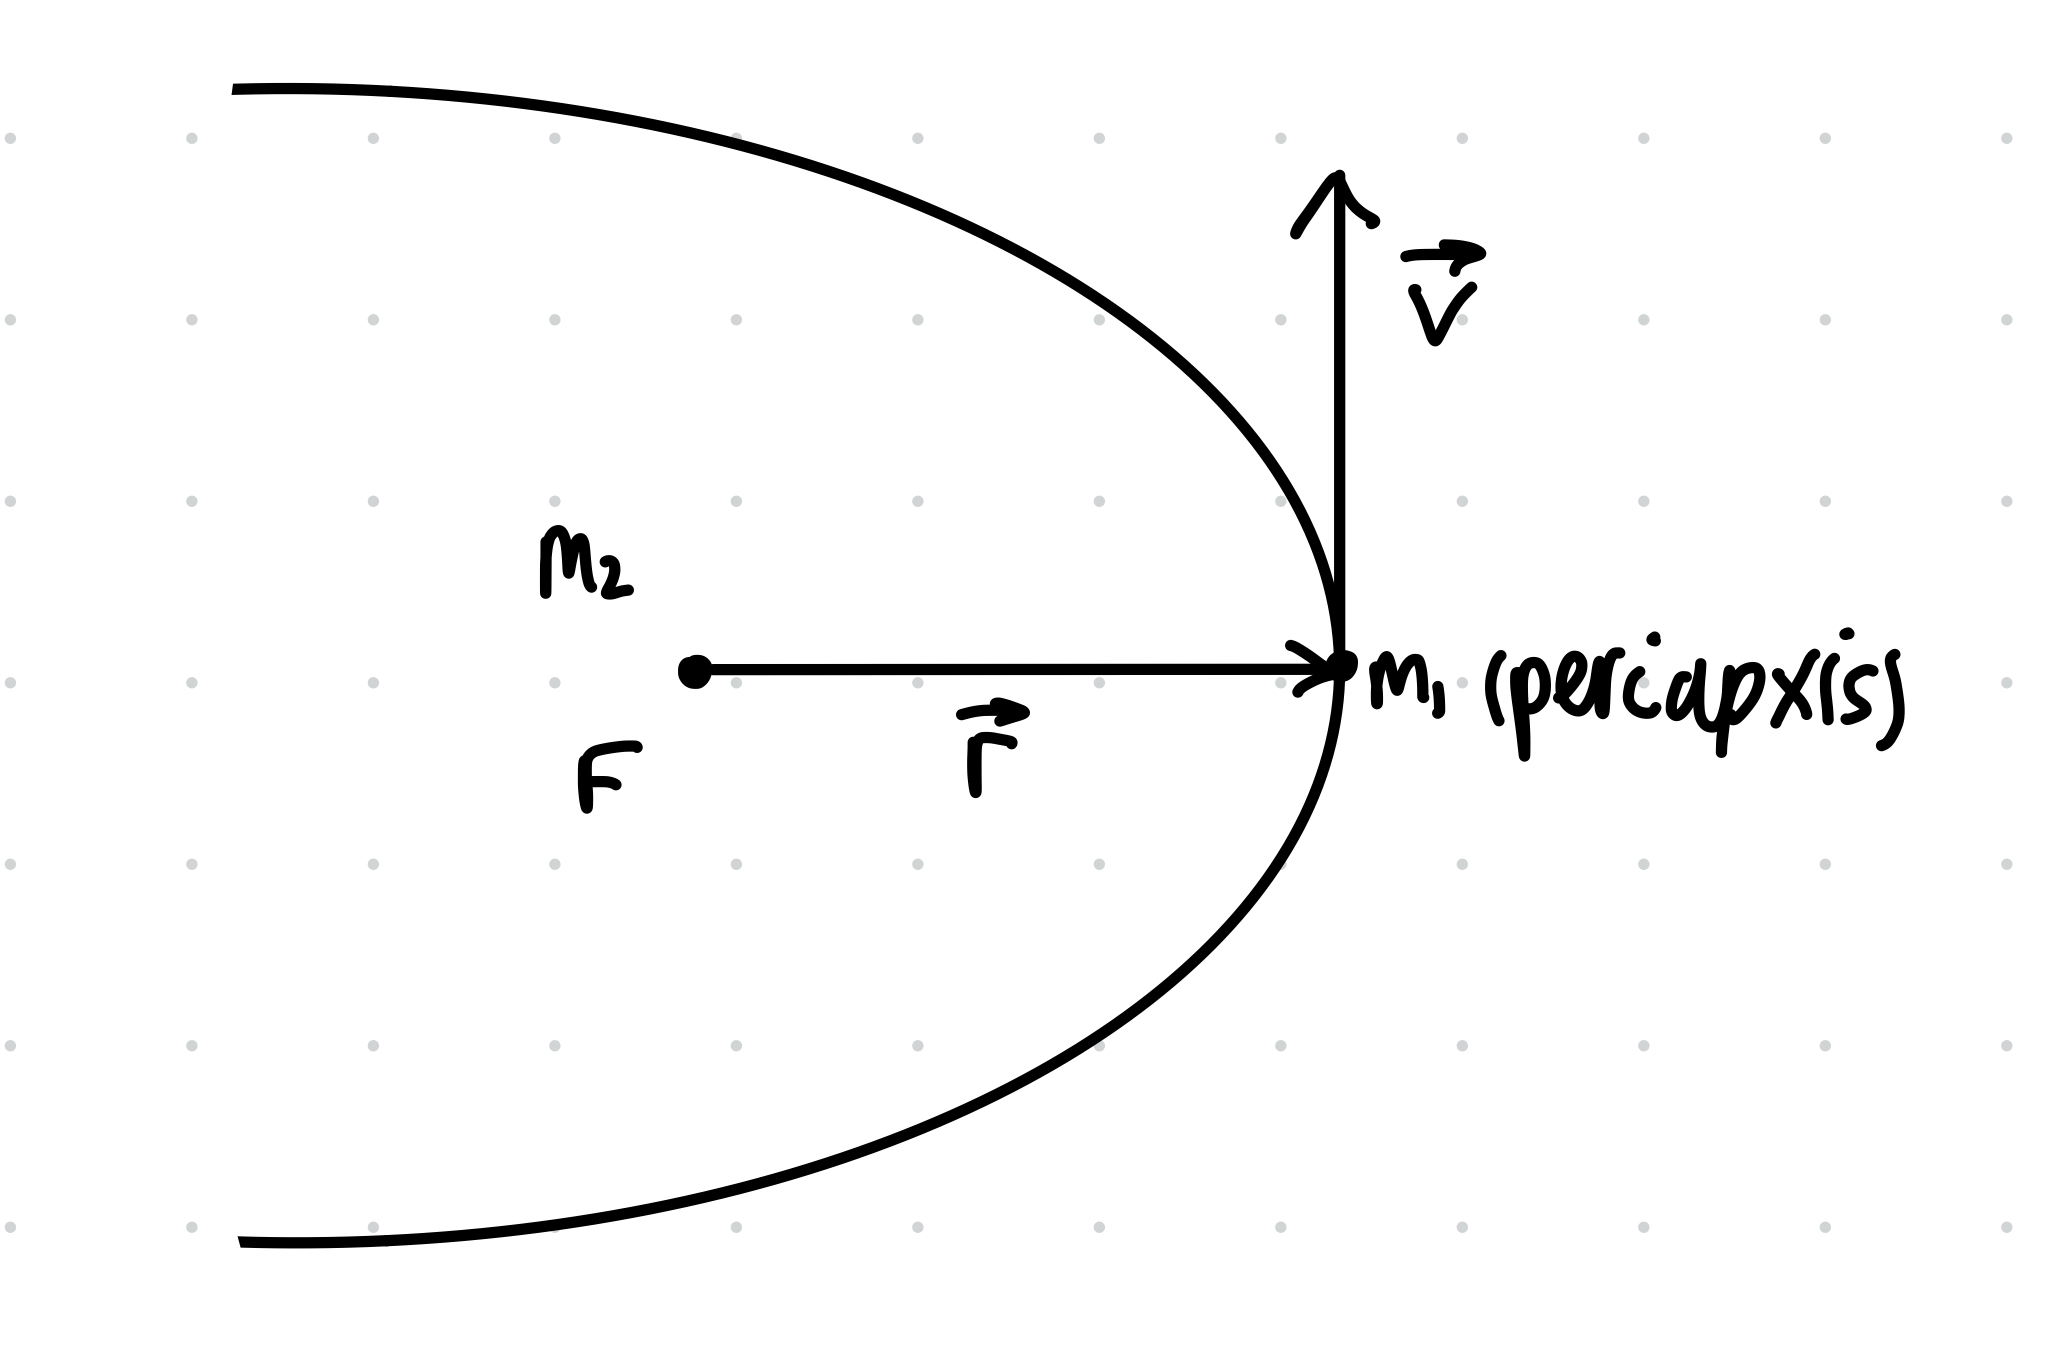
\includegraphics[width=1.0\textwidth]{Cuerpo/Imagenes/02_Ejercicio_1_2.png}
	\end{minipage}

	Tenemos que $\cn=c\hnu_3$ donde $\hnu_3=\hnu_1\wedge\hnu_2$. Supongo que $m_2\gg m_1$. Entonces:

	\begin{equation}
		\rn_c \simeq \rn_2 = 0 \tquad \rn_1 = \rn \tquad \vn = v \hnu_2
	\end{equation}
	Y por tanto $\en=\frac{1}{\mu} (\vn \wedge \cn) - \frac{\rn}{r}$. Ahora hacemos que

	\begin{equation}
		\vn \wedge \cn = \begin{vmatrix}
			\hnu_1 & \hnu_2 & \hnu_3 \\
			0      & v      & 0      \\
			0      & 0      & c
		\end{vmatrix} = v c \hnu_1
	\end{equation}
	Y por tanto:

	\begin{equation}
		\en = \frac{vc}{\mu} \hnu_1 - \hnu_1 \Rightarrow \en = \ccorchetes{\frac{vc}{\mu}-1}\hnu_1
	\end{equation}
	quedando demostrado que lleva el sentido de la periapsis.
\end{texercise}

\begin{texercise}

	El pasado mes de octubre se pudo observar desde nuestra posición geográfica el cometa C/2023 A3 (Tsuchinshan-ATLAS) en su acercamiento en movimiento parabólico al Sistema Solar. Queremos calcular su distancia más cercana al Sol y para ello nos hemos descargado sus efemérides del Small-Body Database (https://ssd.jpl.nasa.gov/horizons/) para el día 12/10/2024 a las 22:00 horas:

	\begin{align*}
		\vec{r} & = (5.3823308478186\times10^{-1}, 9.0771915790989\times10^{-2}, 9.6661892045926\times10^{-2}) \text{ ua}    \\
		\vec{v} & = (1.7983375835632\times10^{-2}, -1.7986317330981\times10^{-2}, 2.0201122328974\times10^{-2}) \text{ ua/d}
	\end{align*}
    Así, obten/responde a las siguientes preguntas:
    \begin{enumerate}[label=\alph*)]
    \item Obtén el perihelio de eeste cometa.
	\item En la misma base de datos se indica que el perihelio es de 0.3914 ua, ¿es la misma que has encontrado? ¿Por qué?
	\end{enumerate}
	Datos: $G = 6.6738 \times 10^{-11} \text{ Nm}^2\text{kg}^{-2} = 1.4881 \times 10^{-34} \text{ ua}^3\text{d}^{-2}\text{kg}^{-1}$. Masa del Sol: $1.989 \times 10^{30}$ kg. [Solución: 2.1.) 0.3787 ua.]
	\tcblower 

	Tenemos la ecuación para conocer el ángulo:

	\begin{equation}
		r(f) = \frac{c^2/ \mu}{1+e\cos(f)}
	\end{equation}
	Cuando $e=1$ tenemos perihelio $f=0$. El valor de $r_p = c^2/2\mu$. El valor de la masa reducida $$\mu=G(m_{\text{sol}}+m_{\text{cometa}})\simeq G m_{\text{sol}} = 2.95\cdot 10^{-4} \ua^3/d$$(ddespreciamos la masa del cometa).Ahora calculamos

	\begin{equation}
		c=|\rn\wedge\vn|=0.015 \*ua^2/
	\end{equation}
	de lo que puedo obtener el valor de $r_p$:
	\begin{equation}
		r_p = \frac{c^2}{2\mu} = 0.379 \ua
	\end{equation}
\end{texercise}

\begin{texercise}
	Marte tiene dos satélites naturales, Phobos y Deimos, que orbitan a su alrededor en órbita elíptica, del mismo modo que Marte orbita alrededor del Sol. Hemos observado que el período orbital de Phobos es de 0.319033 días y su semi-eje mayor es de 9400 km. Sabiendo que el período y semi-eje mayor de Marte son de 686.98 días y $227.956\times10^6$ km, respectivamente, halla la masa de Marte. Dato: Masa del Sol $1.989 \times 10^{30}$ kg. [Solución: $6.46 \times 10^{23}$ kg.]
	\tcblower prueba
\end{texercise}

\begin{texercise}
	La Estación Espacial Internacional (ISS) realiza 15.5 órbitas alrededor de la Tierra en un día y alcanza una altitud sobre la superficie terrestre de 413 km en el perigeo y de 422 km en el apogeo.
    \begin{enumerate}[label=\alph*)]
        \item Halla el semi-eje mayor, la excentricidad y el período de la órbita de la ISS alrededor de la Tierra.
	    \item Calcula las velocidades máxima y mínima alcanzadas.
	    \item Estima la masa de la Tierra. ¿Es el mismo valor que encontramos en las bases de datos?
    \end{enumerate}
	Datos: $G = 6.6738 \times 10^{-11} \text{ Nm}^2\text{kg}^{-2}$, radio medio de la Tierra $R = 6367.44$ km. [Solución: 5.1) $a = 6784.945$ km, $e = 0.00066$, $T = 92.9$ min. 5.2) $v_{\max} = 7777.01$ m/s, $v_{\min} = 7521.52$ m/s. 5.3) $M_T = 5.946912 \times 10^{24}$ kg.]
	\tcblower prueba
\end{texercise}

\tcbstoprecording

\section{{Soluciones}}

\tcbinputrecords
